\documentclass[border=10pt]{standalone}
\usepackage{tikz}
\usetikzlibrary{shapes,arrows,positioning,automata}

\begin{document}

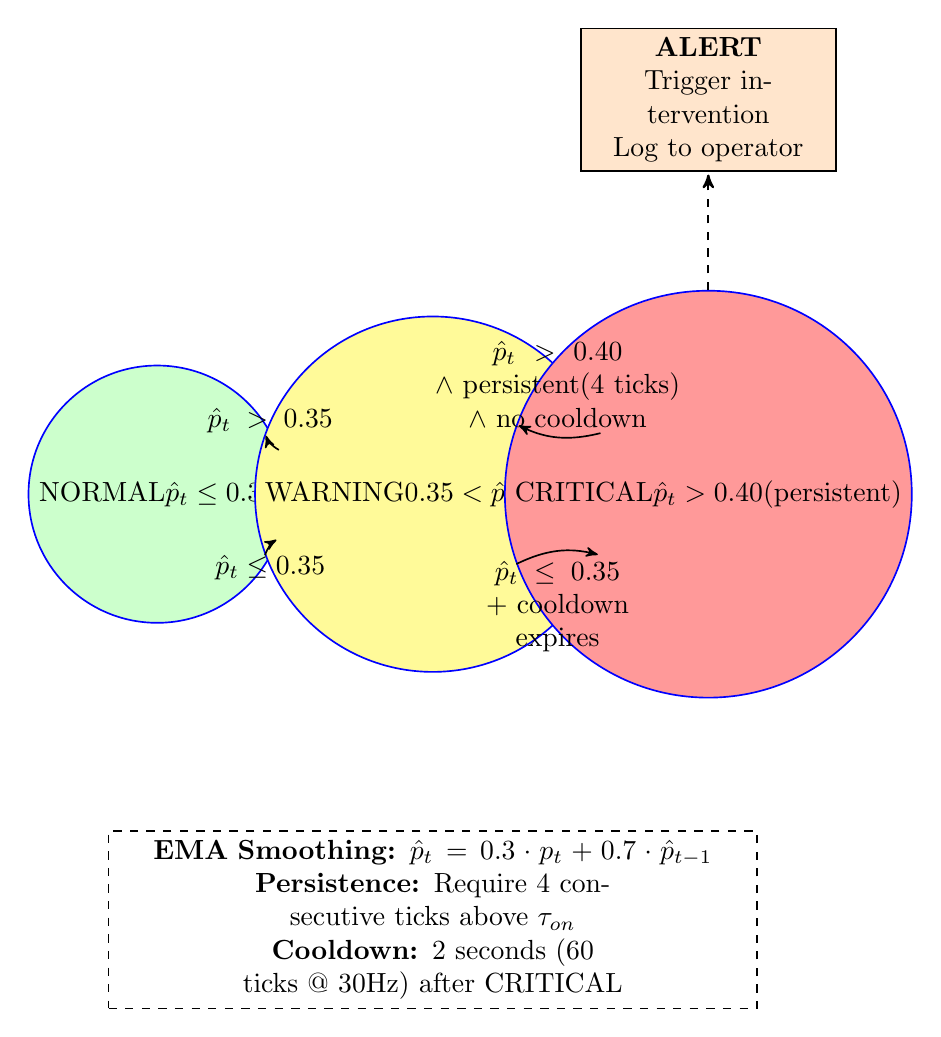
\begin{tikzpicture}[->,>=stealth',shorten >=1pt,auto,node distance=3.5cm,
                    semithick]

  \tikzstyle{every state}=[fill=blue!20,draw=blue,text=black,minimum size=1.5cm]

  \node[state,fill=green!20] (NORMAL) {NORMAL\\$\hat{p}_t \leq 0.35$};
  \node[state,fill=yellow!40,right of=NORMAL] (WARNING) {WARNING\\$0.35 < \hat{p}_t \leq 0.40$};
  \node[state,fill=red!40,right of=WARNING] (CRITICAL) {CRITICAL\\$\hat{p}_t > 0.40$\\(persistent)};

  \path (NORMAL) edge [bend left=20] node[above,text width=3cm,align=center] {$\hat{p}_t > 0.35$} (WARNING)
        (WARNING) edge [bend left=20] node[below] {$\hat{p}_t \leq 0.35$} (NORMAL)
        (WARNING) edge [bend left=20] node[above,text width=3.5cm,align=center] {$\hat{p}_t > 0.40$\\$\land$ persistent(4 ticks)\\$\land$ no cooldown} (CRITICAL)
        (CRITICAL) edge [bend left=20] node[below,text width=3cm,align=center] {$\hat{p}_t \leq 0.35$\\+ cooldown expires} (WARNING);

  % EMA smoothing box
  \node[draw,dashed,rectangle,below=2cm of WARNING,text width=8cm,align=center] (ema) {
    \textbf{EMA Smoothing:} $\hat{p}_t = 0.3 \cdot p_t + 0.7 \cdot \hat{p}_{t-1}$\\
    \textbf{Persistence:} Require 4 consecutive ticks above $\tau_\text{on}$\\
    \textbf{Cooldown:} 2 seconds (60 ticks @ 30Hz) after CRITICAL
  };

  % Alert action box
  \node[draw,rectangle,fill=orange!20,above=1.5cm of CRITICAL,text width=3cm,align=center] (alert) {
    \textbf{ALERT}\\
    Trigger intervention\\
    Log to operator
  };

  \draw[->,thick,dashed] (CRITICAL) -- (alert);

\end{tikzpicture}

\end{document}
